% Created 04-03-2016
% Put the atmospheric graph and drag coefficient graph fit in 19-09-2016
% 15-11-2016 add equations for state, state derivatives, gravity thrust and drag from early versions and used for RKF
% 17-11-2016 Remembered that I have to include a section on the cirularisation. And included the numbers for the speed of sound contant parameters.


\chapter{Models} 
\label{ch:models}
The \ac{MAV} and the corresponding ascent can be modelled in many different ways. Depending on the desired accuracy of the final solution compared to the real-life expected trajectory, different perturbations and freedom in motion can be defined and included, ranging from a low fidelity to a high fidelity program. The main goal of this thesis is to determine if \ac{TSI} is an integrator that can be used for ascent cases and determine its performance compared to previously established methods. Therefore, it should be close to a real-life ascent, but not include too many aspects as to make the problem too complex to test. Therefore, it was decided to design a low fidelity program to propagate the trajectory using accelerations in the x-, y- and z-direction (3DOF). The \ac{MAV} system can then be modelled as a point-mass system with different accelerations acting on it. The change in position can be described by the kinematic equations and the change in velocity by the corresponding dynamic equations. The change in mass is then described by the mass-flow. All these equations are provided in \Cref{sec:stateAndStateDerivatives}. For this model, three perturbing accelerations will be taken into account: the gravity, the thrust and the drag. The effect of third bodies can be neglected because of the short mission time. All the accelerations are described in \Cref{sec:gravityModel,sec:thrustModel,sec:dragModel} respectively. 

\section{State and state derivatives}
\label{sec:stateAndStateDerivatives}
\textbf{\textcolor{red}{Maybe include more assumptions and corresponding explanations!!}}
The general model is described in terms of the Cartesian state; position and velocity in the x-, y-, and z-direction and the mass. The notation is shown in \Cref{eq:stateModel}, where $m_{MAV}$ is the mass of the \ac{MAV} and the subscript $I$ refers to the inertial frame.

\begin{align} \label{eq:stateModel}
\mathbf{r}&=\begin{pmatrix}
x_{I}\\
y_{I}\\
z_{I}\\
\end{pmatrix}
&
\mathbf{V}&=\begin{pmatrix}
V_{x_{I}} \\
V_{y_{I}} \\
V_{z_{I}}\\
\end{pmatrix}
&
m_{MAV}&
\end{align}

In order to determine the next state, the change in the state parameters over time have to be computed. This is done by taking the time derivatives of the state as described by \Cref{eq:state_derivativesModel}.

\begin{align} \label{eq:state_derivativesModel}
\begin{split} 
\dot{x}_{I}&=V_{x_{I}}\\
\dot{y}_{I}&=V_{y_{I}}\\
\dot{z}_{I}&=V_{z_{I}}
\end{split} 
&
\begin{split}
\ddot{x}_{I}&=\dot{V}_{x_{I}}=a_{x_{I}}\\
\ddot{y}_{I}&=\dot{V}_{y_{I}}=a_{y_{I}}\\
\ddot{z}_{I}&=\dot{V}_{z_{I}}=a_{z_{I}}
\end{split}
&
\dot{m}_{MAV}=-\dfrac{T}{g_{0}I_{sp}}
\end{align}

From this point on, the subscript $I$ is omitted, because the state and the state derivatives are always presented in the inertial frame. If variables have to be presented in any other reference frame the corresponding subscripts will be provided and explained. The accelerations in the x-, y- and z-direction have three contributing components: gravitational acceleration, drag acceleration and thrust acceleration. In this model it is assumed that there is a homogeneous gravitational field acting on the point mass with a direction towards the centre of the inertial frame. The gravitational acceleration can therefore be directly expressed in the inertial frame. \\
The drag is assumed to work in the opposite direction of the \ac{MAV} velocity vector, which in turn is assumed to be in the positive x-direction of the body frame associated with the \ac{MAV}. This way the \ac{MAV} velocity, or ground velocity, is acting through the nose of the ascent vehicle. The drag acceleration is therefore expressed in the body frame. This effect in the body frame has to be translated into an acceleration in the inertial frame. This can be done using transformation matrices. A traditional transformation matrix uses an Euler angle to rotate a coordinate frame in a certain reference frame to another. Using the proper Euler, or rotation, angles, the acceleration in the x-, y- and z-direction in the body frame can be transformed into acceleration components acting in the x-, y- and z-direction of the inertial frame. Once it is expressed in the inertial frame it can be added to the effect caused by the gravitational acceleration. \\
It is also assumed that the nozzle of the \ac{MAV} engine can be pivoted in two different directions: the y-, and z-direction of the body frame. This means that the thrust acceleration is not acting directly in the body frame, but in what is called the propulsion frame. Because the nozzle can move in two directions, or rather pivot over two different angles, the thrust acceleration can be translated to the body frame using these two thrust angles. Once the thrust acceleration is expressed in the body frame, the same transformations that are used for the drag can be used to determine the thrust acceleration components in the inertial frame. \\

Combining this in one equation then results in the expression for the acceleration vector as shown by \Cref{eq:accModel}. The subscript $G$ shows that the parameter is a function of the ground velocity. $\mathbb{T}$ stands for a transformation and the subscript determines the rotation axis. The parameter in the brackets for each transformation is the rotation angle. 

\begin{multline} \label{eq:accModel}
\begin{pmatrix}
a_{x}\\
a_{y}\\
a_{z}\\
\end{pmatrix}
=
\begin{pmatrix}
a_{x,Grav}\\
a_{y,Grav}\\
a_{z,Grav}\\
\end{pmatrix}+
\Bigg|_{\mathbf{I}}\mathbb{T}_{\mathbf{z}}\left(-\Omega_{M}t_{O}+\omega_{P}\right)\Bigg|_{\mathbf{R}}\mathbb{T}_{\mathbf{z}}\left(-\tau\right)\mathbb{T}_{\mathbf{y}}\left(\dfrac{\pi}{2}+\delta\right)\Bigg|_{\mathbf{V}}\mathbb{T}_{\mathbf{z}}\left(-\chi_{G}\right)\mathbb{T}_{\mathbf{y}}\left(-\gamma_{G}\right)\Bigg|_{\mathbf{B}}\left[
\begin{pmatrix}
a_{Drag}\\
0\\
0\\
\end{pmatrix}
+  \right. \dots \\
\dotsc
 \left.
\Bigg|_{\mathbf{B}}\mathbb{T}_{\mathbf{z}}\left(-\psi_{T}\right)\mathbb{T}_{\mathbf{y}}\left(-\epsilon_{T}\right)\Bigg|_{\mathbf{P}}
\begin{pmatrix}
a_{Thrust}\\
0\\
0\\
\end{pmatrix}
\right]
\end{multline}

The rotations required to go from the body frame to the inertial frame are all a function of the current state. Both thrust angles are an input value that is set by the user or the program. $-\Omega_{M}t_{O}+\omega_{P}$ represents the angle between the rotating frame and the inertial frame and consists of three parts. $\Omega_{M}$ is the rotational velocity of Mars around it's own axis, $t_{O}$ is the difference between the current time and the time at which the inertial frame was set on Mars, and $\omega_{P}$ is the angle between the x-axis of the inertial frame and the zero meridian at the time that the inertial frame was set on Mars. In this thesis the inertial frame is set at the beginning of the simulation (so at $t=0$, $t_{O}=0$) and is aligned with the rotating frame (so $\omega_{P}=0$). The transformation from the vertical to the rotating frame requires the latitude and longitude of the \ac{MAV}, which is a function of the current state. \cite{mooij1994motion} provides equations to determine the different rotation angles. These expressions can be used to compute the latitude and longitude as well as shown by \Cref{eq:latAndLong}.

\begin{align} \label{eq:latAndLong}
\begin{split} 
r&=\sqrt{x^{2}+y^{2}+z^{2}}\\
\delta&=\arcsin\left(\dfrac{z}{r}\right)
\end{split} 
&
\begin{split}
x_{R}&=\cos\left(\Omega_{M}t_{O}\right)x+\sin\left(\Omega_{M}t_{O}\right)y\\
y_{R}&=-\sin\left(\Omega_{M}t_{O}\right)x+\cos\left(\Omega_{M}t_{O}\right)y\\
\tau&=\text{atan2}\left(\dfrac{y_{R}}{x_{R}}\right)
\end{split}
\end{align}
 
It can be seen that in order to compute the longitude in the rotating frame ($\tau$) the position of the \ac{MAV} in the rotating frame was required. This position was found by transforming the inertial position to the rotational position using $\Omega_{M}t_{O}$ as described before. Working out that transformation matrix results in the sines and cosines presented in \Cref{eq:latAndLong}.\\

Similarly, the flight-path angle and the azimuth angle can be described as a function of the current state. For this, some intermediate parameters have to be computed first and are given by \Cref{eq:intermediateParameters}.

\begin{equation} \label{eq:intermediateParameters}
\begin{split}
V_{I}=&\sqrt{V_{x}^{2}+V_{y}^{2}+V_{z}^{2}}\\
V_{G}=&\sqrt{V_{I}^{2}+\Omega_{M}^{2}\left(x^{2}+y^{2}\right)+2\Omega_{M}\left(xy-yx\right)}\\
V_{x,V}=&\left(V_{x}+\Omega_{M}y\right)\cdot \left(\sin\left(\delta\right)\sin\left(\Omega_{M}t_{O}\right)\sin\left(\tau\right)-\cos\left(\Omega_{M}t_{O}\right)\cos\left(\tau\right)\sin\left(\delta	\right)\right)+\\
&\left(V_{y}-\Omega_{M}x\right)\cdot \left(-\cos\left(\tau\right)\sin\left(\delta\right)\sin\left(\Omega_{M}t_{O}\right)-\cos\left(\Omega_{M}t_{O}\right)\sin\left(\delta\right)\sin\left(\tau\right)\right)+V_{z}\cos\left(\delta\right)\\
V_{y,V}=&\left(V_{x}+\Omega_{M}y\right)\cdot \left(-\cos\left(\tau\right)\sin\left(\Omega_{M}t_{O}\right)-\cos\left(\Omega_{M}t_{O}\right)\sin\left(\tau\right)\right)+\\
&\left(V_{y}-\Omega_{M}x\right)\cdot \left(\cos\left(\Omega_{M}t_{O}\right)\cos\left(\tau\right)-\sin\left(\Omega_{M}t_{O}\right)\sin\left(\tau\right)\right)\\
V_{z,V}=&\left(V_{x}+\Omega_{M}y\right)\cdot \left(\cos\left(\delta\right)\sin\left(\Omega_{M}t_{O}\right)\sin\left(\tau\right)-\cos\left(\Omega_{M}t_{O}\right)\cos\left(\tau\right)\cos\left(\delta	\right)\right)+\\
&\left(V_{y}-\Omega_{M}x\right)\cdot \left(-\cos\left(\tau\right)\cos\left(\delta\right)\sin\left(\Omega_{M}t_{O}\right)-\cos\left(\Omega_{M}t_{O}\right)\cos\left(\delta\right)\sin\left(\tau\right)\right)-V_{z}\sin\left(\delta\right)\\
\end{split}
\end{equation}

Then the angles can be computed using those parameters as shown by \Cref{eq:fpaAndazimuth}.


\begin{equation} \label{eq:fpaAndazimuth}
\begin{split}
\chi_{G}&=\text{atan2}\left(\dfrac{V_{y,V}}{V_{x,V}}\right)\\
\gamma_{G}&=-\arcsin\left(\dfrac{V_{z,V}}{V_{G}}\right)\\
\end{split}
\end{equation}

In this case, a transformation from the inertial frame to the vertical frame was required to get information on the velocity in the vertical frame. This transformation is written out at sines and cosines in \Cref{eq:intermediateParameters} resulting in lengthy expressions. \\

Now that the rotation angles from the body frame to the inertial frame are known, only the thrust angles and the different accelerations have yet to be defined. This is done in the next sections.


\section{Gravity}
\label{sec:gravityModel}
The gravity acceleration is a function of the position of the \ac{MAV} and the standard gravitational parameter of the planet, in this case Mars. Often, irregularities in the mass distribution of a planet also have to be taken into account ($J_{2,0}$ etc.), however, because the mission time is very short and the \ac{MAV} does not even complete one revolution around Mars, these effects can be neglected. Therefore, the gravitational acceleration in the inertial frame can be represented by \Cref{eq:gravityModel}.

\begin{equation} \label{eq:gravityModel}
\begin{pmatrix}
a_{x,Grav}\\
a_{y,Grav}\\
a_{z,Grav}\\
\end{pmatrix}
=
\begin{pmatrix}
-\mu_{M}\dfrac{x}{r^{3}}\\
-\mu_{M}\dfrac{y}{r^{3}}\\
-\mu_{M}\dfrac{z}{r^{3}}\\
\end{pmatrix}
\end{equation}


\section{Thrust}
\label{sec:thrustModel}
The thrust acceleration in the propulsion frame is simply the thrust divided by the current mass of the \ac{MAV}, which can be written as shown by \Cref{eq:thrustModel}.

\begin{equation} \label{eq:thrustModel}
a_{Thrust}=\dfrac{T}{m_{MAV}}
\end{equation}

However, this acceleration has to be transformed to the body frame using the thrust angles. These thrust angles are the thrust elevation ($\epsilon_{T}$) and thrust azimuth ($\psi_{T}$) angle, and are defined in \Cref{fig:propframe_mooij1994motion}.

\begin{figure}[!ht]
\centering
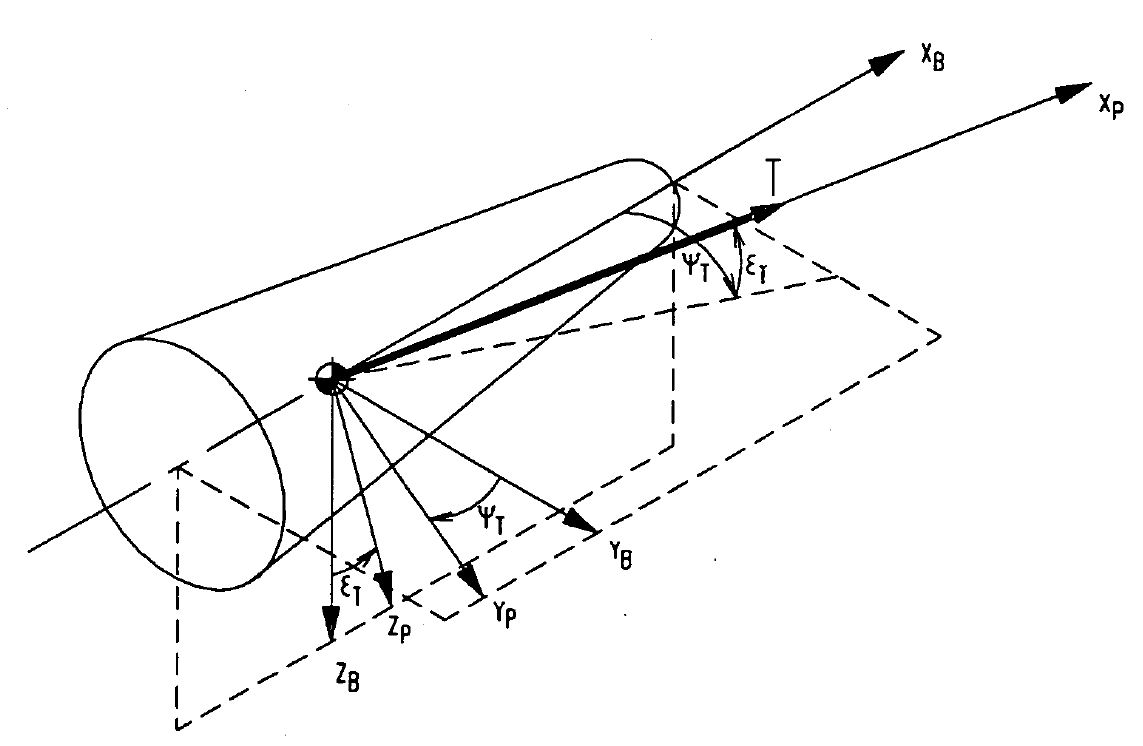
\includegraphics[width=0.8 \textwidth]{figures/reference_frames/propframe_mooij1994motion.jpg}
\caption{Definition of the thrust elevation and thrust azimuth angle with respect to the body frame \citep{mooij1994motion}.}
\label{fig:propframe_mooij1994motion}
\end{figure}

These angles will not be computed, but are set as an input for the program.


\section{Drag}
\label{sec:dragModel}
The drag acceleration can be represented similarly to the thrust acceleration taking into account that the drag is acting in the negative x-direction in the body frame. The acceleration can then be written as \Cref{eq:dragModel}.

\begin{equation} \label{eq:dragModel}
a_{drag}=-\dfrac{D}{m_{MAV}}
\end{equation}

Here the drag is given by \Cref{eq:dragDragModel}.

\begin{equation} \label{eq:dragDragModel}
D=\dfrac{1}{2}\rho V_{G}^{2}SC_{D}
\end{equation}

Where $S$ is the reference area of the \ac{MAV} set by the user, $\rho$ is the air density which is a function of the altitude $h\left(=r-R_{MOLA}\right)$ and $C_{D}$ is the drag coefficient of the \ac{MAV} which is a function of the Mach number. The Mach number in turn is a function of the speed of sound, which depends on the air temperature as can be seen in \Cref{eq:machAndSpeedOfSound}.

 \begin{equation} \label{eq:machAndSpeedOfSound}
\begin{split}
M &= \dfrac{V_{G}}{a} \\
a &= \sqrt{\gamma_{a}R_{a}^{*}T_{a}} \quad \text{where} \quad R_{a}^{*}=\dfrac{R_{a}}{M_{a}} \\
\end{split}
\end{equation}

Here, $R_{a}$ is the molar gas constant, $\gamma_{a}$ is the adiabetic index for Mars, which according to \cite{ho2002radio} can be set as $\sim$1.35. $M_{a}$ is the molecular mass of the Martian atmosphere and depends on it's composition. \cite{williams2015} mentions a volumetric composition of Mars which results in a mean molecular mass of 0.04334 kg/mol. This value has been used in this research to compute the speed of sound.\\

The air pressure and temperature ($T_{{a}}$) change as a function of the altitude of the \ac{MAV}. This means that a pressure and temperature model of the atmosphere of Mars will have to be used to approximate these values as the ascent vehicle moves through the atmosphere. This is done through a function fit of an atmospheric model, as is described in \Cref{subsec:atmofuncfit}.\\

The drag coefficient changes with the Mach number, however, this change is not constant over the entire Mach range. Therefore, this also requires a function fit in order to be used in the simulation program. This fit is presented in \Cref{subsec:dragCoefFuncFit}.

\subsection{Atmospheric graph function fit}
\label{subsec:atmofuncfit}
Using Mars-\ac{GRAM} 2005, a table containing altitude, latitude and longitude dependent temperature and density data was produced. The altitude range was -0.6 to 320 km \ac{MOLA} with a step-size of 0.01 km, the latitude and longitude ranges were centred around the launch site (21.0 $^\circ$N and 74.5 $^\circ$E) with a 10 degree range in each direction and a step-size of 1 degree. The rest of the input parameters were constant and can be seen in \Cref{app:appendixA-marsGRAM-inputFile}. The temperature and density data produced is shown in \Cref{fig:temperatureData,fig:densityData} respectively for 9 latitude and longitude combinations including the launch site itself.                                                                                                                                                                                                                                                                                                                                                                                                                                                                                          


\begin{figure}[!ht]
\centering
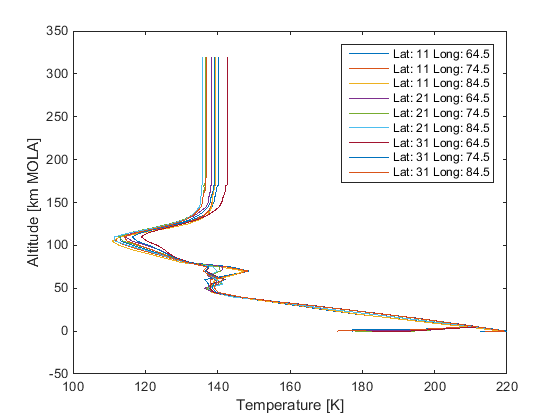
\includegraphics[width=1.0\textwidth]{figures/software/temperatureData.png}
\caption{Temperature data generated with Mars-\ac{GRAM} 2005 showing 9 different latitude and longitude combinations}
\label{fig:temperatureData}
\end{figure}

\begin{figure}[!ht]
\centering
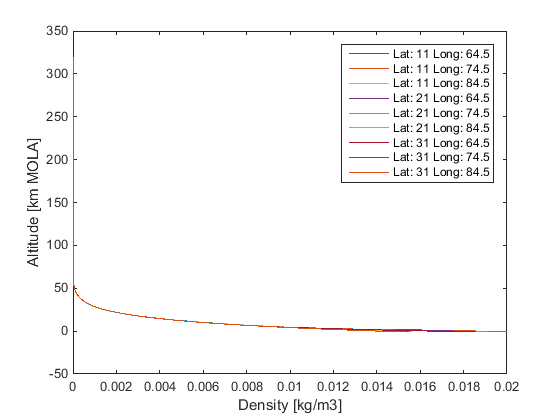
\includegraphics[width=1.0\textwidth]{figures/software/densityData.png}
\caption{Density data generated with Mars-\ac{GRAM} 2005 showing 9 different latitude and longitude combinations}
\label{fig:densityData}
\end{figure}

Unfortunately discontinuous data tables cannot be used when integrating using \ac{TSI}, which is why both these data tables had to be fitted with continuous functions. The temperature data could not be smoothly fit with one continuous function.  Therefore, depending on the altitude range, a different approximation function is required. The condition to be met for a proper fit came from the differences in the temperature-altitude and density-altitude curves, where the maximum difference with respect to the launch site curve was taken. The requirement for the standard deviation of the polynomial curve fit was then to be (at least) one order lower than this maximum difference and that the maximum difference between the fit and the launch site curve was lower than the maximum difference. The temperature-altitude curve was split into 5 sections as roughly visualised in \Cref{fig:temperatureDataSplit5}. The number of sections come from both the shape of the curves and the requirement for accuracy and maximum order of the polynomial, which is set at 8 because otherwise the polynomial would get too long. Also, the number of sections were to be kept at a minimum. More information on the fitting process and early results is provided in \Cref{app:appendixB-fittingProcessAndResults}.

\begin{figure}[!ht]
\centering
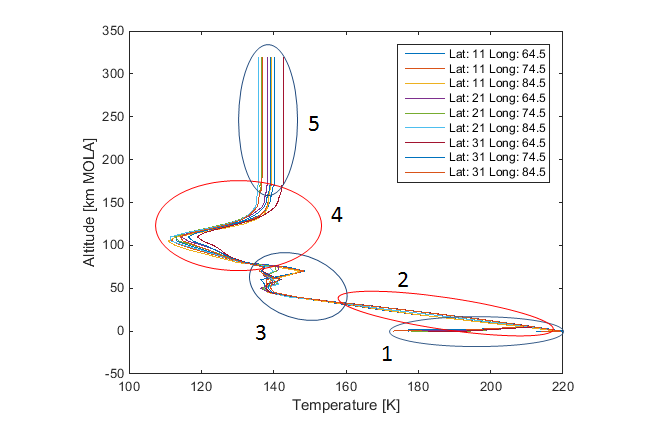
\includegraphics[width=1.0\textwidth]{figures/software/temperatureDataSplit5.png}
\caption{Different temperature curve sections}
\label{fig:temperatureDataSplit5}
\end{figure}

Each section was fit with a polynomial function of the n$^{th}$ order where the function is represented by \Cref{eq:polyGenFunct}. The last section shows a constant temperature, thus the temperature of the launch site curve was chosen to represent this final section, which is equal to 136.5 K.

\begin{equation} \label{eq:polyGenFunct}
y=p_{n}x^{n}+p_{n-1}x^{n-1}+\dots+p_{1}x+p_{0}
\end{equation}

A lower order is preferred, because then the fitted function will be simpler to evaluate and contain fewer terms. However the order has to be high enough to meet the accuracy requirements. \Cref{tab:fitDeviations} shows the orders that were required and the deviations to the launch site temperature-altitude curve. The actual corresponding parameters are provided in \Cref{tab:fitParameters}. It should be noted that the first few temperature data values were so different from the rest of the curve that it was assumed that this is a lack of the Mars-\ac{GRAM} program and were thus treated as outliers.

\begin{table}[!ht]
\begin{center}
\caption{Temperature curve fit data all with respect to the launch site curve (Latitude and longitude of the launch site)}
\label{tab:fitDeviations}
\begin{tabular}{|l|l|l|p{3cm}|p{3cm}|p{3cm}|}
\hline 
\textbf{Section} & \textbf{Altitude range [km MOLA]} & \textbf{Order}	& \textbf{Maximum polynomial standard deviation [K]} & \textbf{Maximum polynomial difference [K]} & \textbf{Maximum data curves difference [K]} \\ \hline 
1 & -0.6 to 5.04 & 1 & 0.0312 & 25.8 & 0.177 \\ \hline
2 & 5.04 to 35.53 & 2 & 0.287 & 3.90 & 0.7056 \\ \hline
3 & 35.53 to 75.07 & 6 & 0.624 & 8.00 & 1.69 \\ \hline
4 & 75.07 to 170.05 & 8 & 0.523 & 6.60 & 2.45 \\ \hline
\end{tabular}
\end{center}
\end{table}

\begin{table}[!ht]
\begin{center}
\caption{Temperature curve fit parameters (rounded to 3 decimal points)}
\label{tab:fitParameters}
\begin{tabular}{|l||p{1.1cm}|p{1.1cm}|p{1.1cm}|p{1.1cm}|p{1.1cm}|p{1.1cm}|p{1.1cm}|p{1.1cm}|p{1.1cm}|}
\hline 
\textbf{Section}  & $\mathbf{p_{8}}$ & $\mathbf{p_{7}}$ & $\mathbf{p_{6}}$ & $\mathbf{p_{5}}$ & $\mathbf{p_{4}}$ & $\mathbf{p_{3}}$ & $\mathbf{p_{2}}$ & $\mathbf{p_{1}}$ & $\mathbf{p_{0}}$ \\ \hline 
1 &  &  &  &  &  &  & & 3.415 & 194.165   \\ \hline
2 &  &  &  &  &  & & 0.006 & -2.130 & 222.052   \\ \hline
3  &  &  & -5.388 $\cdot$10$^{-7}$ & 1.785 $\cdot$10$^{-4}$ & -0.0243 & 1.733 & -68.294 & 1.407 $\cdot$10$^{3}$ & -1.167 $\cdot$10$^{4}$ \\ \hline
4  & 4.1942 $\cdot$10$^{-12}$ & -4.328 $\cdot$10$^{-9}$ & 1.931 $\cdot$10$^{-6}$ & -4.862 $\cdot$10$^{-4}$ & 0.076 & -7.405 & 447.378 & -1.523 $\cdot$10$^{4}$ & 2.236 $\cdot$10$^{5}$ \\ \hline
\end{tabular}
\end{center}
\end{table}

The complete polynomial fit for the launch site curve for the temperature is shown in \Cref{fig:completePolyFitTempSplit5}.

\begin{figure}[!ht]
\centering
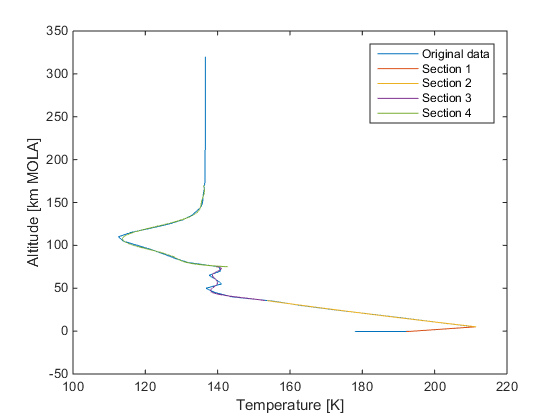
\includegraphics[width=1.0\textwidth]{figures/software/completePolyFitTempSplit5.png}
\caption{All section fits for the launch site temperature data curve}
\label{fig:completePolyFitTempSplit5}
\end{figure}




The density fit was slightly more difficult because the curves are all very similar and thus result in a higher accuracy requirement for the fit. At first glance it looks like a natural logarithmic function, unfortunately an ordinary exponential did not fit the curve. This is why a more extensive exponential fit was required. The natural logarithm of the data has been plotted in \Cref{fig:lnPlotDataDen}.

\begin{figure}[!ht]
\centering
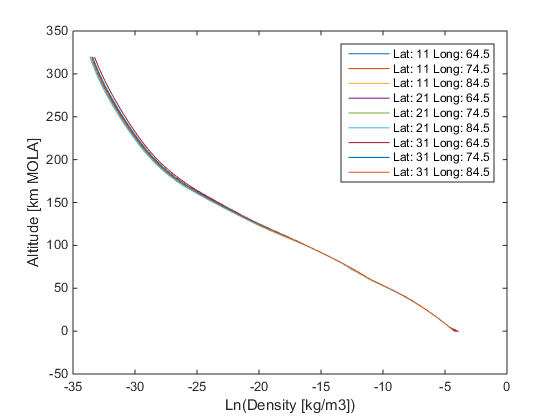
\includegraphics[width=1.0\textwidth]{figures/software/lnPlotDataDen.png}
\caption{Natural logarithmic plot of the density data}
\label{fig:lnPlotDataDen}
\end{figure}

With the data represented in the logarithmic domain, again a polynomial function can be fit. The total fit would then satisfy \Cref{eq:expPoly}.

\begin{equation} \label{eq:expPoly}
y=exp\left( p_{n}x^{n}+p_{n-1}x^{n-1}+\dots+p_{1}x+p_{0}\right)
\end{equation}



% A logarithmic fit (such as an exponential atmosphere) resulted in a lower overall accuracy than the polynomial fits. In this case the curve was split into three sections, because the differences between the curves were bigger in the lower atmosphere. These sections are illustrated in \Cref{fig:densityDataSplit3}.
%
% \begin{figure}[!ht]
%\centering
%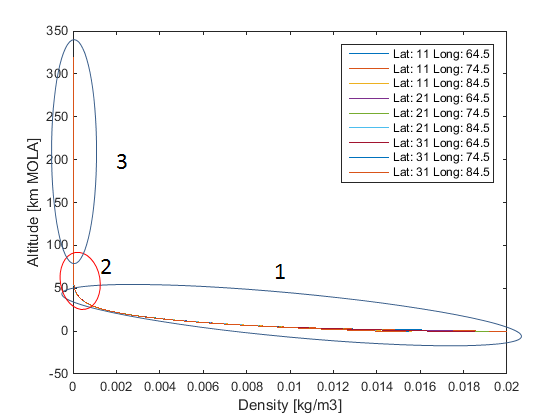
\includegraphics[width=1.0\textwidth]{figures/software/densityDataSplit3.png}
%\caption{Different density curve sections}
%\label{fig:densityDataSplit3}
%\end{figure} 

The same polynomial requirements as for the temperature curve were enforced for the density curve as well. However, because the polynomial is used in an exponential, some extra requirements are needed to assure the accuracy of the fit. One requirement is that the maximum difference between the final exponential fit and the normal launch site density curve is smaller than the maximum difference between all the data curves. Also, in this case the standard deviation of the difference between the exponential fit and the normal launch site curve had to be within the range of standard deviations of the difference between the different data curves. This meant that even though an 8$^{th}$ order polynomial fit could be achieved for the natural logarithmic data with the required accuracy, when converted to the exponential fit, the last two requirements were not met. Before it was mentioned that an order higher than 8 was not desirable. However, in this case, a single exponential fit could be achieved using a 10$^{th}$ order polynomial. This fit meant that the density curve did not have to be split up at all, which makes the integration slightly easier. Therefore, it was decided that a 10$^{th}$ order polynomial was acceptable in this case. The results of the fit is presented in \Cref{tab:fitDeviationsDen,tab:fitParametersDen} and the polynomial and exponential fit curves are shown in \Cref{fig:completeExpPolyFitDen,fig:completeExpFitDen} respectively.

%
% This results in the density polynomial fit data and the polynomial parameters as presented in \Cref{tab:fitDeviationsDen,tab:fitParametersDen} respectively. 

%\textbf{\textcolor{red}{UPDATE THE NEXT TWO TABLE VALUES TO THE VALUES FOR DENSITY!!!}}

%\begin{table}[!ht]
%\begin{center}
%\caption{Density curve fit data (10$^{th}$ order polynomial)}
%\label{tab:fitDeviationsDen}
%\begin{tabular}{|p{3cm}|p{3cm}|p{3cm}|p{3cm}|p{3cm}|p{3cm}|p{3cm}|}
%\hline 
%\textbf{Maximum polynomial standard deviation [kg/m$^{3}$]} & \textbf{Maximum natural logarithmic curves difference [kg/m$^{3}$]} & \textbf{Maximum polynomial difference with natural logarithmic launch site curve [kg/m$^{3}$]} & \textbf{Maximum curves difference [kg/m$^{3}$]} & \textbf{Maximum difference with launch site curve [kg/m$^{3}$]} & \textbf{Maximum standard deviation curves difference [kg/m$^{3}$]} & \textbf{Standard deviation exponential fit difference [kg/m$^{3}$]} \\ \hline 
%0.0501 & 0.460 & 0.160   & 3.910$\cdot$10$^{-3}$ &  2.826$\cdot$10$^{-3}$ & 2.106$\cdot$10$^{-4}$ & 1.167$\cdot$10$^{-4}$ \\ \hline
%
%\end{tabular}
%\end{center}
%\end{table}

\begin{table}[!ht]
\begin{center}
\caption{Density curve fit data (10$^{th}$ order polynomial) with respect to the launch site curve (Latitude and longitude of the launch site)}
\label{tab:fitDeviationsDen}
\begin{tabular}{|l|l|}
\hline 
\textbf{Maximum polynomial standard deviation [kg/m$^{3}$]} & 0.0501 \\ \hline

  \textbf{Maximum polynomial difference [kg/m$^{3}$]} & 0.160 \\ \hline
  
   \textbf{Maximum natural logarithmic data curves difference [kg/m$^{3}$]} & 0.460 \\ \hline
  
    \textbf{Maximum exponential difference with launch site curve [kg/m$^{3}$]} & 2.826$\cdot$10$^{-3}$ \\ \hline
    
       \textbf{Maximum data curves difference [kg/m$^{3}$]} & 3.910$\cdot$10$^{-3}$ \\ \hline
    
      \textbf{Standard deviation exponential fit difference [kg/m$^{3}$]} & 1.167$\cdot$10$^{-4}$ \\ \hline 
      
           \textbf{Maximum standard deviation data curves difference [kg/m$^{3}$]} & 2.106$\cdot$10$^{-4}$ \\ \hline
\end{tabular}
\end{center}
\end{table}



\begin{table}[!ht]
\begin{center}
\caption{Density curve fit parameters (rounded to 3 decimal points)}
\label{tab:fitParametersDen}
\begin{tabular}{|p{1.1cm}|p{1.1cm}|p{1.1cm}|p{1.1cm}|p{1.1cm}|p{1.1cm}|p{1.1cm}|p{1.1cm}|p{1.1cm}|p{1.1cm}|p{1.1cm}|}
\hline 
 $\mathbf{p_{10}}$ & $\mathbf{p_{9}}$ & $\mathbf{p_{8}}$ & $\mathbf{p_{7}}$ & $\mathbf{p_{6}}$ & $\mathbf{p_{5}}$ & $\mathbf{p_{4}}$ & $\mathbf{p_{3}}$ & $\mathbf{p_{2}}$ & $\mathbf{p_{1}}$ & $\mathbf{p_{0}}$ \\ \hline 
2.287 $\cdot$10$^{-21}$  & -3.724 $\cdot$10$^{-18}$ & 2.559 $\cdot$10$^{-15}$ & -9.620 $\cdot$10$^{-13}$ & 2.146 $\cdot$10$^{-10}$ & -2.884 $\cdot$10$^{-8}$ & 2.273 $\cdot$10$^{-6}$ & -9.604 $\cdot$10$^{-5}$ & 1.414 $\cdot$10$^{-3}$ & -0.0962 & -4.172\\ \hline
\end{tabular}
\end{center}
\end{table}

%The complete polynomial fit for the launch site curve for the density is shown in \Cref{fig:completePolyFitDen}.


\begin{figure}[!ht]
\centering
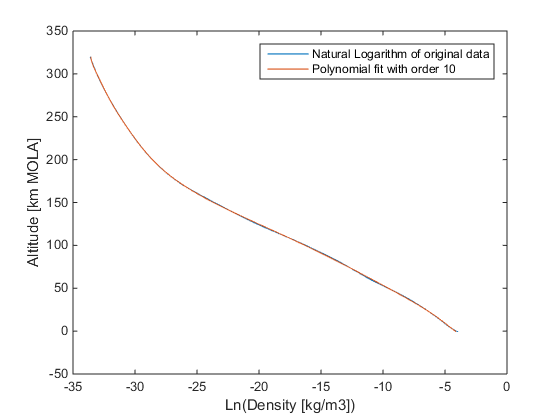
\includegraphics[width=1.0\textwidth]{figures/software/completeExpPolyFitDen.png}
\caption{Polynomial fit for the launch site density data curve}
\label{fig:completeExpPolyFitDen}
\end{figure}

\begin{figure}[!ht]
\centering
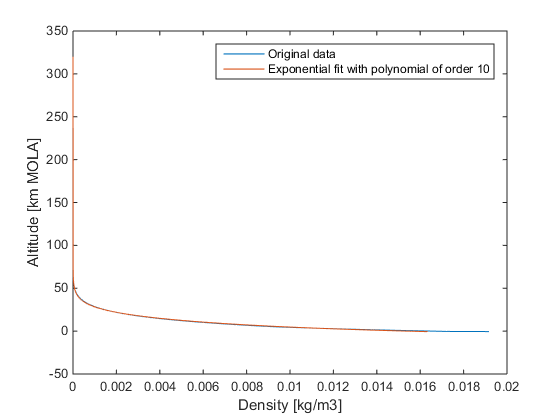
\includegraphics[width=1.0\textwidth]{figures/software/completeExpFitDen.png}
\caption{Exponential fit for the launch site density data curve}
\label{fig:completeExpFitDen}
\end{figure}


%\begin{figure}[!ht]
%\centering
%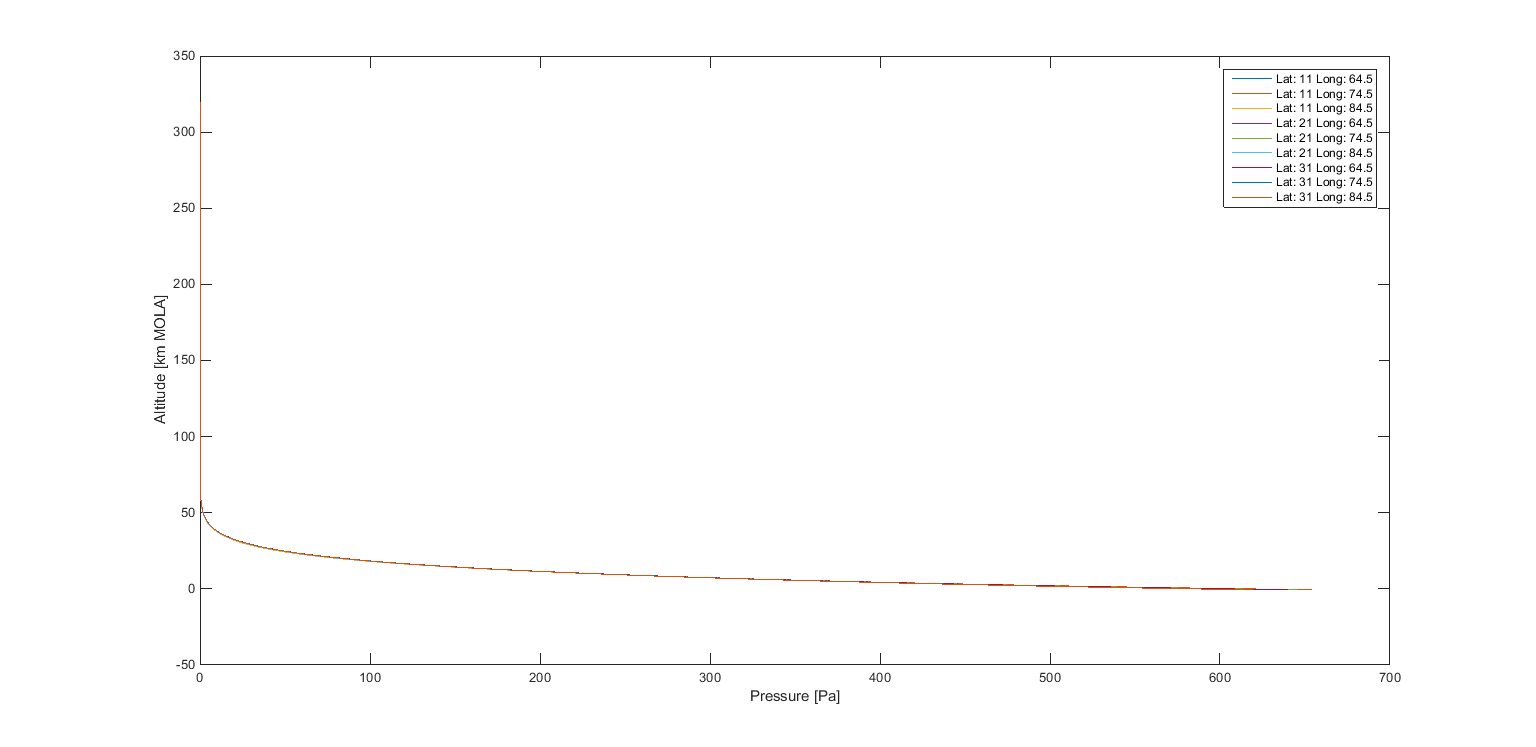
\includegraphics[width=1.0\textwidth]{figures/software/pressureData.png}
%\caption{Pressure data generated with Mars-\ac{GRAM} 2005 showing 9 different latitude and longitude combinations}
%\label{fig:pressureData}
%\end{figure}

\subsection{Drag coefficient graph function fit}
\label{subsec:dragCoefFuncFit}
Similar to the temperature and density curves, the relation between Mach number and drag coefficient, as depicted in \Cref{fig:dragcoeff_whitehead2004mars}, had to be modelled as a continuous function as well. Again, it could not be fitted using one continuous function, but instead had to be modelled by different functions. \\


Fortunately, this curve is already an approximation and thus consists of linear elements only. It can be split up into 6 different sections where the first and last section are constant ($C_{D}$ is 0.2 and 0.3 respectively). Using a similar polynomial fit as before, but now for 1 order only, a linear fit could be made for each of the remaining 4 sections. The corresponding parameters are shown in \Cref{tab:dragCoeffPara} and the curve fit is shown in \Cref{fig:dragCoeffFit}.


\begin{table}[!ht]
\begin{center}
\caption{Drag coefficient curve fit parameters (rounded to 3 decimal points)}
\label{tab:dragCoeffPara}
\begin{tabular}{|l|l||l|l|}
\hline 
\textbf{Section}  & \textbf{Mach range}& $\mathbf{p_{1}}$ & $\mathbf{p_{0}}$ \\ \hline 
2  & 0.5 to 1  & 0.400 & -2.483 $\cdot$10$^{-16}$  \\ \hline
3  & 1 to 1.3  & 0.567 & -0.167  \\ \hline
4  &  1.3 to 2.5 & -0.142 & 0.754 \\ \hline
5  &  2.5 to 4 & -0.0667 & 0.567 \\ \hline
\end{tabular}
\end{center}
\end{table}



\begin{figure}[!ht]
\centering
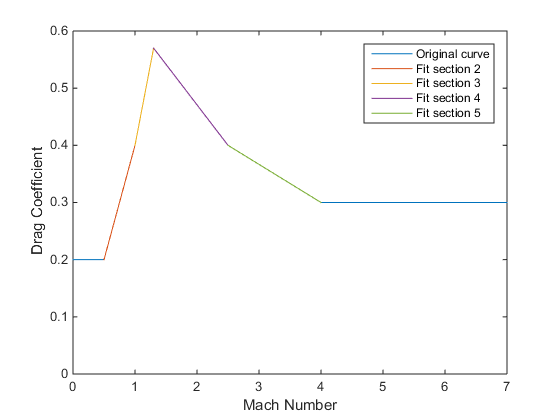
\includegraphics[width=1.0\textwidth]{figures/software/dragCoeffFit.png}
\caption{All section fits for the drag coefficient - Mach curve}
\label{fig:dragCoeffFit}
\end{figure}

\section{Circularisation}
\label{sec:modelCircularisation}
\textbf{\textcolor{red}{This section still has to be added!!}}